\begin{frame}{Redes Neurais Convolucionais}
	\begin{itemize}
		\item Redes \emph{feedfoward} com muitas camadas ocultas
		\medskip
		\item Cada camada possui uma funcionalidade b�sica espec�fica e produz um \alert{mapa de caracter�sticas}
		\medskip
		\item Realiza��o de opera��es de convolu��o
		\begin{itemize}
			\item Extra��o de caracter�sticas por meio de um filtro
			\item Par�metros: extens�o espacial, \emph{stride}, \emph{zero-padding}, etc
		\end{itemize}
		\medskip
		\item Camada \emph{pooling} respons�vel por produzir um mapa de caracter�sticas condensado
		\medskip
		\item Camadas completamente conectadas baseadas nos conceitos de uma rede \alert{\emph{Multilayer Perceptron}}
	\end{itemize}
\end{frame}

\begin{frame}{Redes Neurais Convolucionais}
	\begin{figure}[!ht]
		\centering
		\label{img:lenet}
		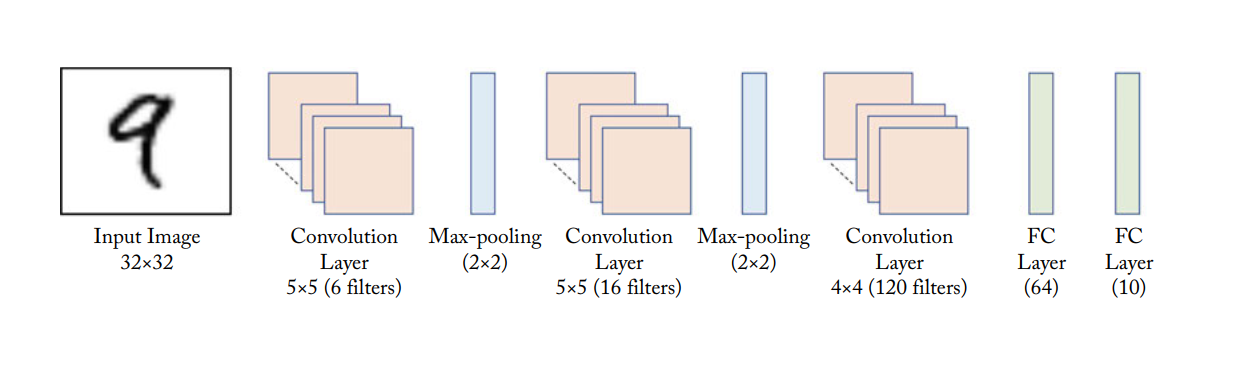
\includegraphics[width=1\textwidth]{./img/lenet}
	\end{figure}
\end{frame}

\begin{frame}{Arquiteturas Can�nicas de Redes Neurais Convolucionais}
	\begin{itemize}
		\item Desafio anual desenvolvido pelo projeto ImageNet
		\item \emph{ImageNet Large Scale Visual Recognition Challenge} (ILSVRC)
		\bigskip
		\item T�m promovido algumas arquiteturas de CNNs bem sucedidas em determinados problemas
		\bigskip
		\item ISLVRC 2014
		\begin{itemize}
			\item 2� lugar: VGGNet - pequenos filtros
			\item 1� lugar: GoogLeNet - \emph{Inception Module}
		\end{itemize}
		\bigskip
		\item Vencedora do ILSVRC 2015: ResNet - blocos residuais
	\end{itemize}
\end{frame}

\begin{frame}{Arquiteturas Can�nicas de Redes Neurais Convolucionais}
	\begin{figure}[!ht]
		\centering
		\label{img:vggnet}
		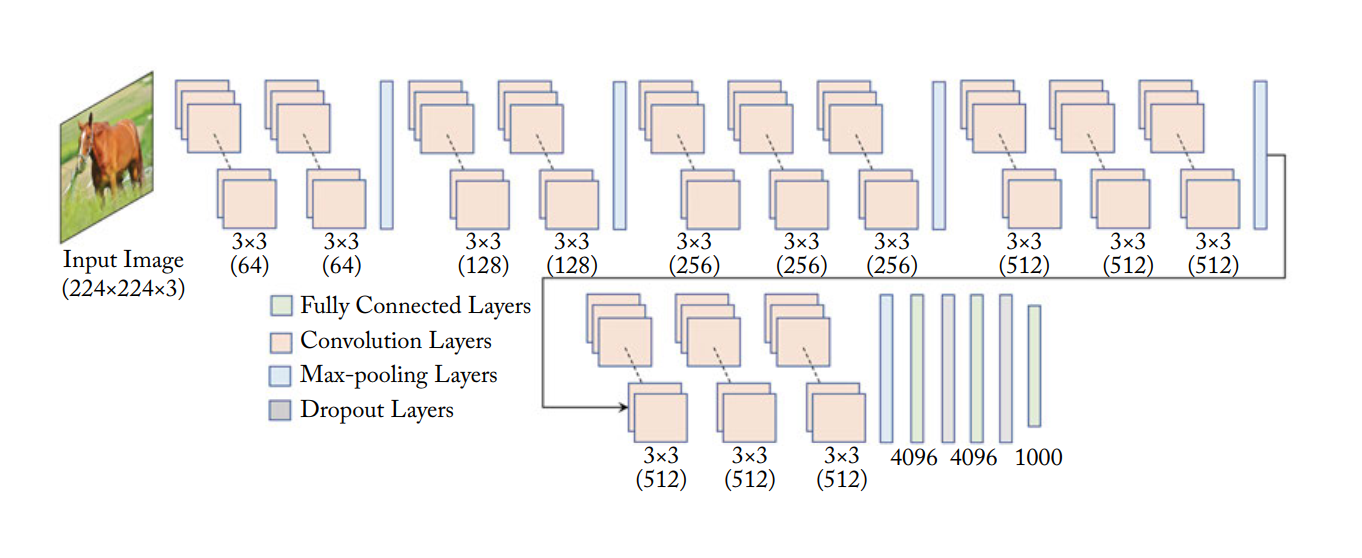
\includegraphics[width=1\textwidth]{./img/vggnet}
	\end{figure}
\end{frame}

\begin{frame}{\emph{Transfer Learning}}
	\begin{itemize}
		\item Permite utilizar uma rede pr�-treinada e adapt�-la a um novo conjunto de dados
		\bigskip
		\item Modelos treinados com um conjunto gen�rico de dados conseguem capturar caracter�sticas universais
		\bigskip
		\item Treinamentos com conjuntos de dados bastante conhecidos
		\begin{itemize}
			\item ImageNet
			\item Places50
		\end{itemize}
		\bigskip
		\item Modifica��o na camada de sa�da para obter o aprendizado desejado
	\end{itemize}
\end{frame}